%----------
%	PRUEBA DE CONCEPTO DE APLICABILIDAD EDITORIAL
%----------

La finalidad última del sistema no es puntuar en una evaluación, sino asistir el
trabajo de análisis sobre el corpus, incluidas las miles de piezas sin anotar.
Para materializar esa aplicabilidad, el sistema de detección se integra en la
\textbf{herramienta web del proyecto IRIS}~\cite{avi2026}\footnote{\url{https://dei.inf.uc3m.es/iris/} [Último acceso: 05/08/2026]},
y la prueba de concepto consiste en usar esa herramienta para acompañar a expertas
y periodistas en el análisis de un corpus de prueba.

La asistencia cubre los dos planos del análisis de contenido experto
(Sección~\ref{sec:experts}). En el plano \textbf{cuantitativo}, la herramienta agrega
las etiquetas que produce el sistema en informes por variable, con tablas de
frecuencias y porcentajes sobre el conjunto seleccionado y un análisis descriptivo
automático (Figura~\ref{fig:iris-web-informe}), lo que permite explorar qué medios,
secciones o periodos concentran más usos marcados. En el plano \textbf{cualitativo},
para cada pieza muestra el marcado de las evidencias sobre el texto y la explicación
del veredicto (Figura~\ref{fig:iris-web-analisis}), de modo que quien analiza puede
leer por qué el sistema ha decidido lo que ha decidido.

El sistema no automatiza la decisión: la produce en un formato revisable (código,
justificación y evidencias literales) y la analista acepta, rechaza o matiza cada
veredicto.

Los resultados del Capítulo~\ref{results_and_discussion} obligan a matizar el
alcance. El acuerdo entre el sistema y las anotadoras es bajo, y buena parte de ese
desacuerdo podría tener que ver con lo amplio y variable del criterio experto más que con
un fallo de detección. Por eso la herramienta no se plantea como un clasificador
autónomo, sino como un
\textbf{apoyo a la postedición}: en lugar de sustituir el criterio editorial, se
inserta en el flujo de trabajo de quien revisa un texto ya redactado. El sistema
señala las piezas candidatas y aporta en cada caso las evidencias y la
justificación del veredicto, de modo que la analista edita ese diagnóstico
(lo acepta, lo rechaza o lo matiza) en segundos y con plena trazabilidad, en vez
de partir de cero.

Las Figuras~\ref{fig:iris-web-informe} y~\ref{fig:iris-web-analisis} ilustran ambas
vistas de la herramienta web, la de informe cuantitativo y la de análisis por pieza.

\begin{figure}[H]
    \centering
    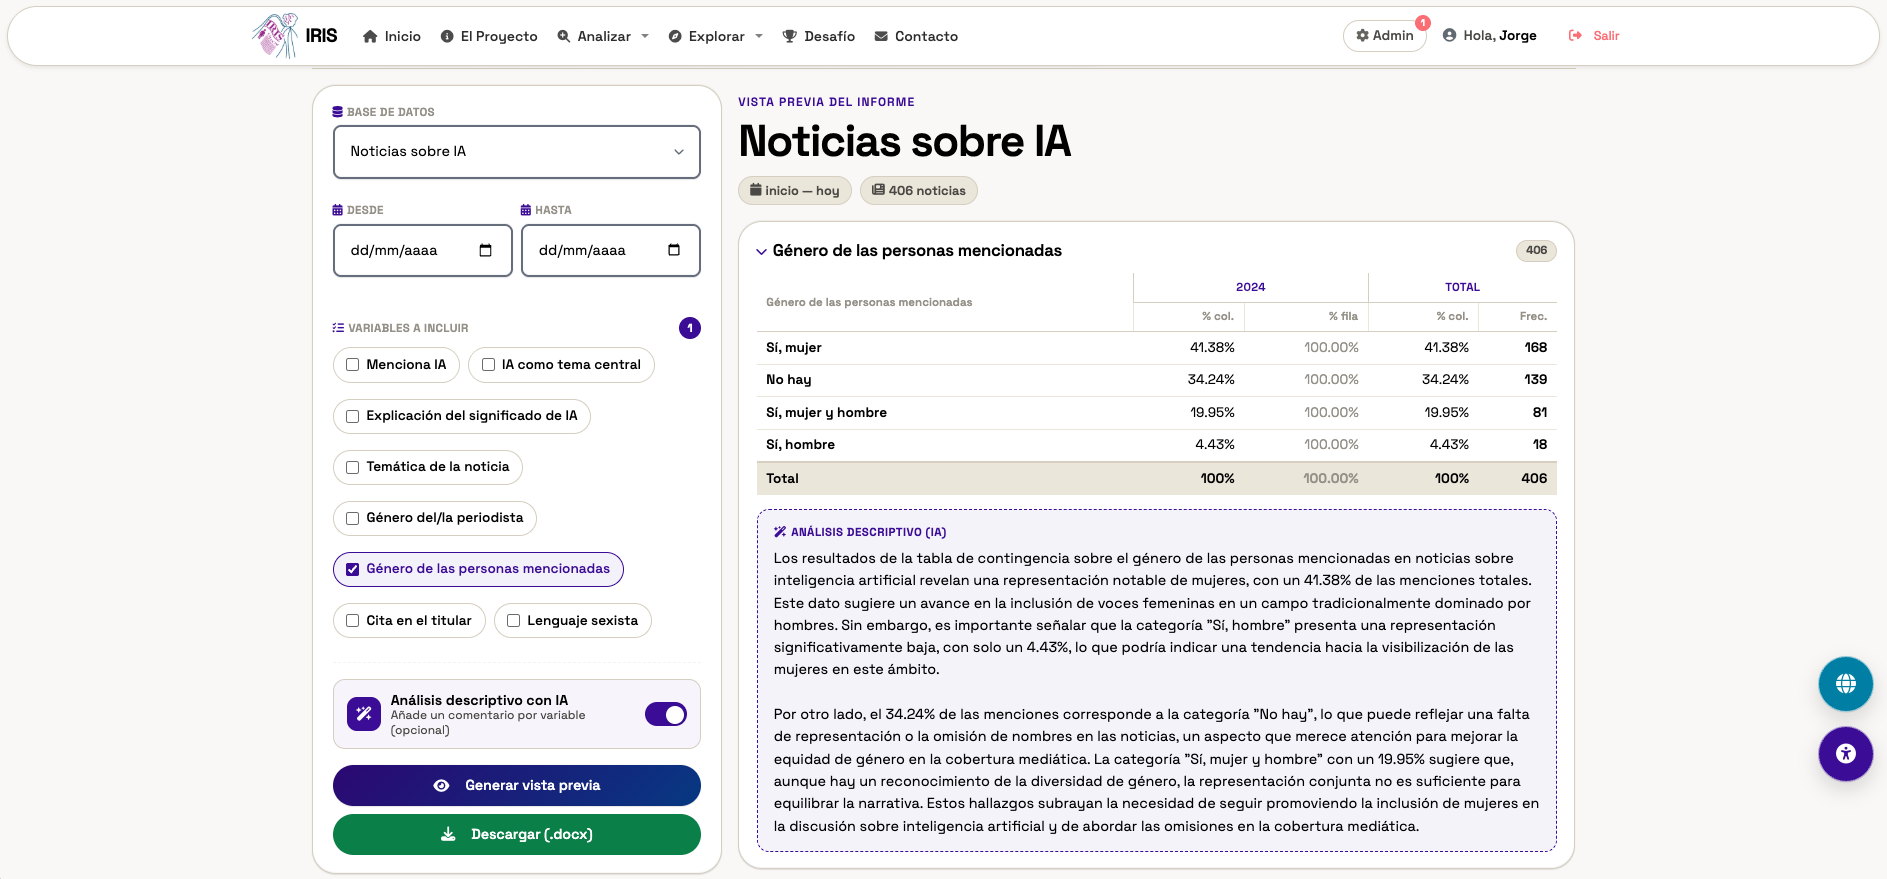
\includegraphics[width=\textwidth]{Plantilla_TFG_ingles_2019/imagenes/iris_3.png}
    \caption{Vista de informe cuantitativo en la herramienta web del proyecto IRIS.
    Para las variables seleccionadas genera tablas de frecuencias y porcentajes sobre
    el conjunto de piezas, acompañadas de un análisis descriptivo automático.}
    \label{fig:iris-web-informe}
\end{figure}

\begin{figure}[H]
    \centering
    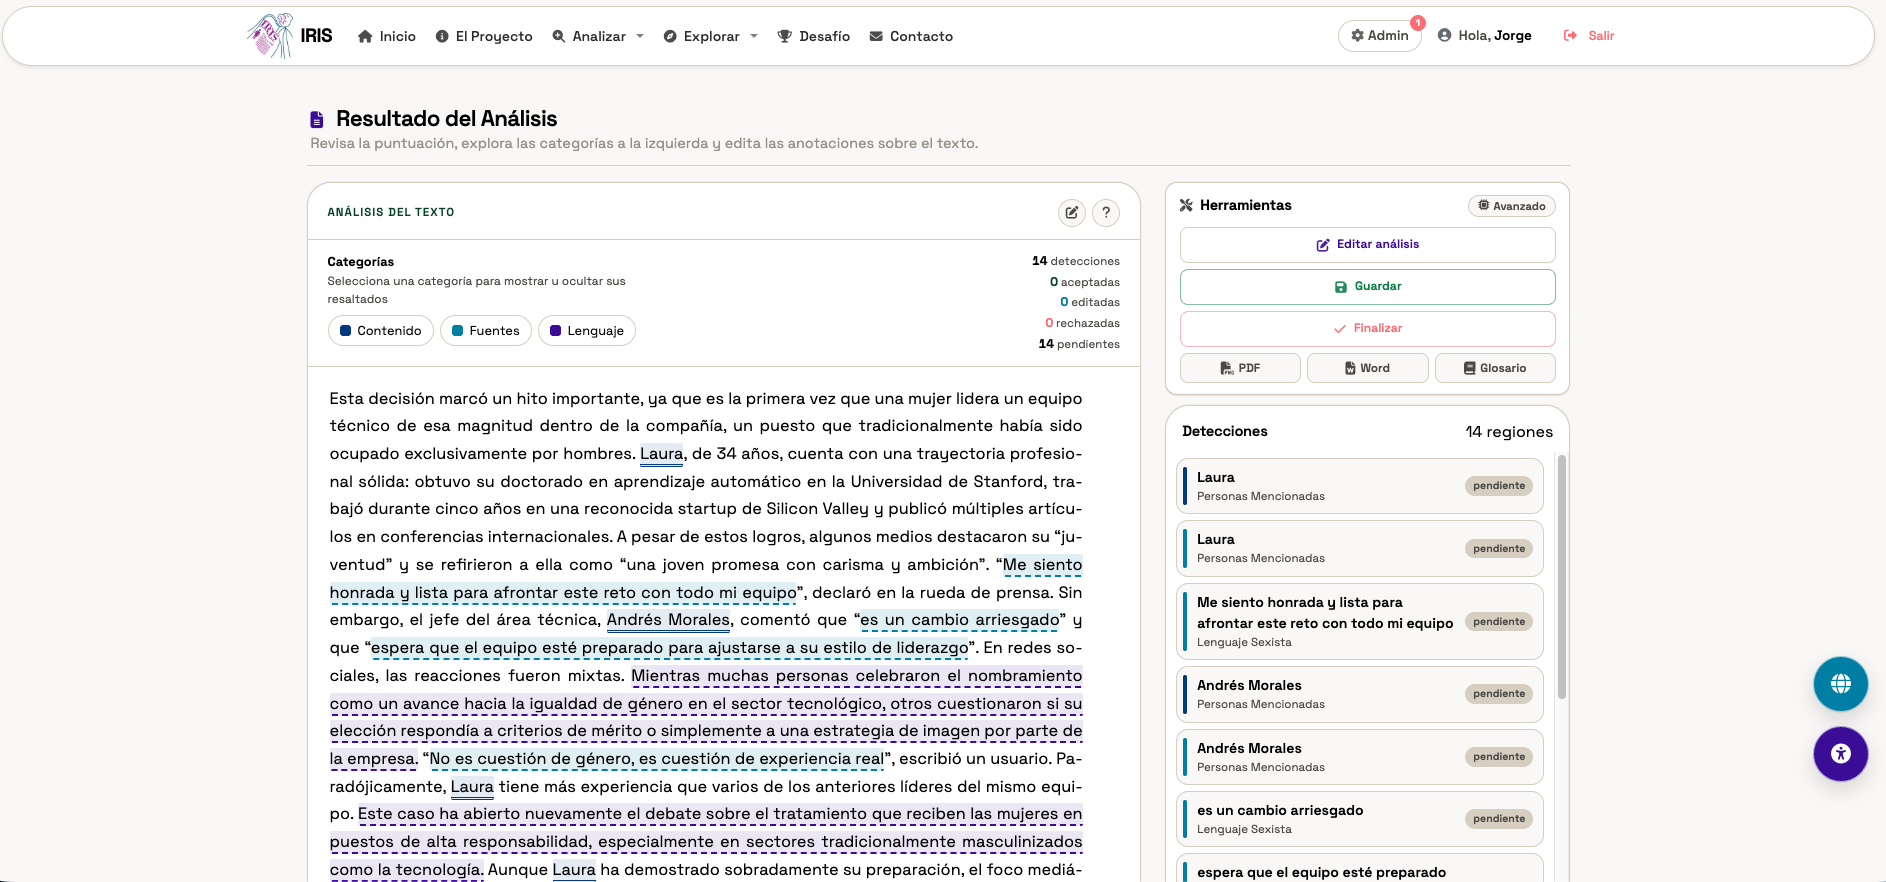
\includegraphics[width=\textwidth]{Plantilla_TFG_ingles_2019/imagenes/iris_2.png}
    \caption{Vista de resultado del análisis en la herramienta web del proyecto IRIS.
    Las detecciones se resaltan sobre el texto y se listan por categoría, con los
    controles para que la analista acepte, edite o rechace cada una (postedición con
    la persona en el bucle).}
    \label{fig:iris-web-analisis}
\end{figure}
